\section{Your Proposed Method}\label{sec:yourmethod}

% Now comes the ``beef'' of the paper, where you explain what you did. Again,
% organize it in paragraphs with titles. As in every section you start with a
% very brief overview of the section.

% For this course, explain all the optimizations you performed. This mean, you
% first very briefly explain the baseline implementation, then go through
% locality and other optimizations, and finally SSE (every project will be
% slightly different of course). Show or mention relevant analysis or
% assumptions. A few examples: 1) Profiling may lead you to optimize one part
% first; 2) bandwidth plus data transfer analysis may show that it is memory
% bound; 3) it may be too hard to implement the algorithm in full generality:
% make assumptions and state them (e.g., we assume $n$ is divisible by 4; or, we
% consider only one type of input image); 4) explain how certain data accesses
% have poor locality. Generally, any type of analysis adds value to your work.

% As important as the final results is to show that you took a structured,
% organized approach to the optimization and that you explain why you did what
% you did.

% Mention and cite any external resources including library or other code.

% Good visuals or even brief code snippets to illustrate what you did are good.
% Pasting large amounts of code to fill the space is not good.

In this section we define the scope of our implementation, describe the baseline
implementation and its bottlenecks and outline the steps which were followed to
increase the performance. At the end the remaining performance blockers.

\mypar{Basic implementation}
Our implementation uses an iterative quadtree approach. We consider only grayscale image of squared sizes of powers of two.
Algorithm \ref{alg:baseline} illustrates the compression of the algorithm, whose inputs are the image (row-wise array of doubles) of size $S \times S$, 
the max quadtree depth $m$ and the error threshold $\epsilon$.\\
The function \textsc{partition($image$,$s$)} partitions the image into contiguous non-overlapping blocks of size $s \times s$.
The function \textsc{quad($R_i$, $s$)} takes a range block of size $s \times s$ and partitions it into 4 smaller range blocks.
The function \textsc{compute($image$,$R_i$, $D_i$)} computes a transformation with and the resulting RMS according to section \ref{sec:background}. 
Note that the function implicitly rotates the domain block, i.e. the function looks at the four possible locations and returns the transformation with the smallest error.
\begin{algorithm}
\caption{Compression using iterative quadtree}\label{alg:baseline}
\hspace*{\algorithmicindent} \textbf{Input:} $img$ (image of size $S \times S$), $\epsilon$ (RMS threshold) \\
\hspace*{\algorithmicindent} \textbf{Output:} $\boldsymbol{T}$ (set of computed transformations)
\begin{algorithmic}[1]
  \State $\boldsymbol{T} \gets \{\}$ \Comment{Learned transformations} 
  \State $\boldsymbol{R} \gets \Call{partition}{img, S/2}$ \Comment{Initial range blocks} 
    \For{$c=1..m$} \Comment{$c$ is the current quadtree depth}
        \State $\boldsymbol{D} \gets \Call{partition}{img, S/2^{c-1}}$
        \For{$R_i \in \boldsymbol{R}$}
            \State $err_i \gets \infty, T_i \gets \NULL$
            \For{$D_i \in \boldsymbol{D}$}
              \State $T_x, err_x \gets $ \Call{compute}{$img$, $D_i$, $R_i$}
              \If{$err_x < err_i$}
                \State $T_i \gets T_x$
                \State $err_i \gets err_x$
              \EndIf
            \EndFor
        \EndFor
        \State $\boldsymbol{R} \gets \boldsymbol{R} \backslash  R_i$ \Comment{Remove $R_i$ from $\boldsymbol{R}$}
        \If{$err_i > \epsilon$}
          \State $\boldsymbol{R} \gets \boldsymbol{R} \cup  \Call{quad}{R_i, S/2^c}$
        \Else
          \State $\boldsymbol{T} \gets \boldsymbol{T} \cup \{T_i\}$
        \EndIf
    \EndFor
\end{algorithmic}
\end{algorithm}

\mypar{Scope} For our implementation only square grayscale images with a power
of two width and height were considered. The reason for the restriction on the
size is that it simplifies \textit{Quadtree Partitioning}. If the width of a
range block is a power of two and no suitable transformation is found for it,
then the four new range blocks created by dividing the original range block into
4 equal parts will also have a power of two width. Colored images can be
compressed and decompressed in the same manner as grayscale images.

\notepascal{are we sure about the color stuff?}

\mypar{Baseline Implementation} An overseeable Python implementation and the C
code of Y.Fischer were used as a reference for the baseline implementation.

\notepascal{not sure what to write here :/}
\notepascal{cite python and fischer implementation}

\mypar{Profiling} With Valgrind's callgrind and cachegrind

\mypar{Bandwidth and Data Transfer}

\begin{figure}
  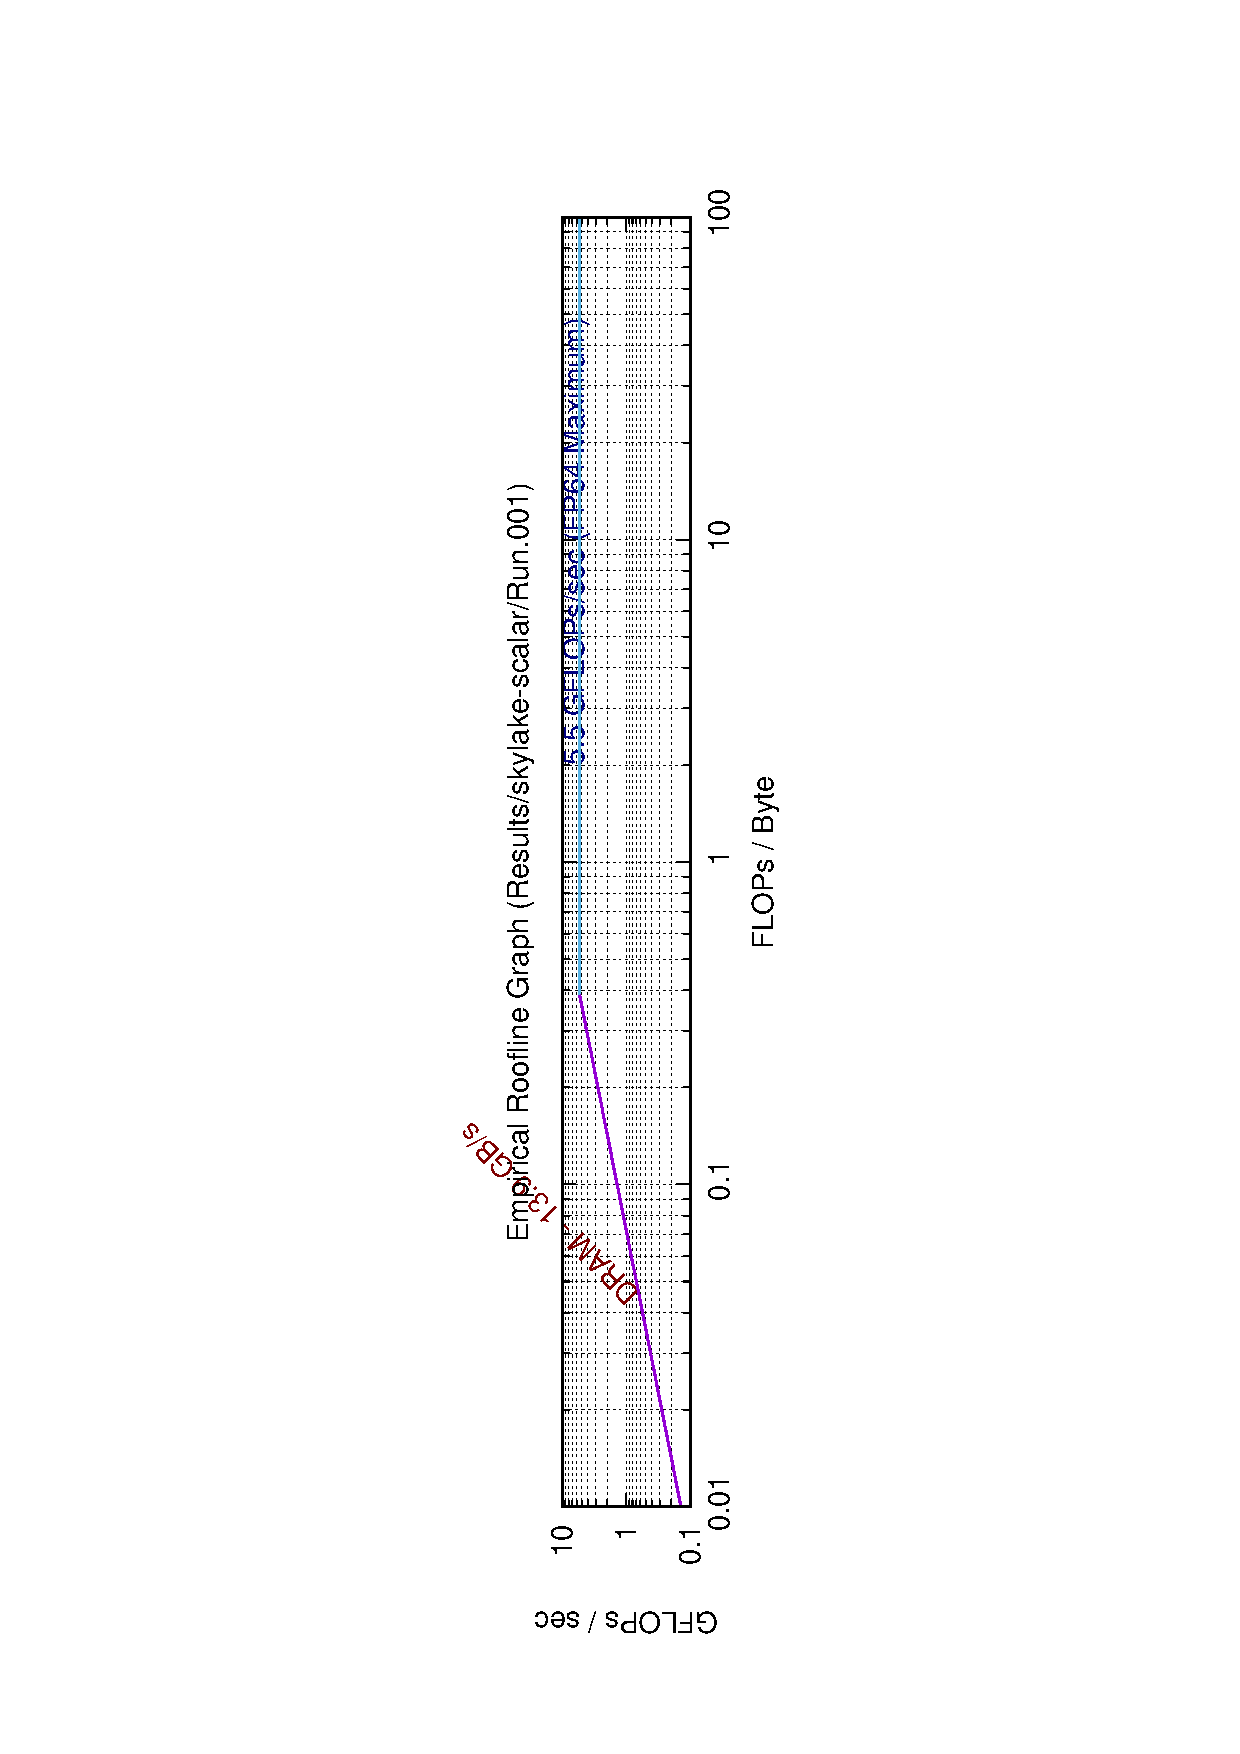
\includegraphics[page=1, width=.45\textwidth]{roofline}
  \caption{Roofline}
\end{figure}

\mypar{Scalar Optimizations}

\mypar{Vector Optimizations}

\mypar{Block Rotations}

\mypar{Srided Access}
